\chapter{Design Options}\label{ch:design_options}
This chapter presents the design configuration generation process that has been undertaken, to come up with several feasible design concepts and configurations that shall be further investigated throughout this project.
As such, this chapter presents a Design Option Tree (DOT) with all the possible proposed configurations, after which each branch of the Tree is detailed, and exclusion criteria of different configurations are made clear based on preliminary calculations and engineering judgement.

\section{Design Option Tree}
A DOT was made in \Cref{fig:DOT} and is split up into four branches: Fixed-wing structure, Transwing, Rotorcraft and Canard.
Each of these branches is subdivided into additional sub-branches.
The branches end up in concepts, where each concept is shown with an identifier in a purple box.
Some of the concepts are discarded, if a concept is discarded because it is infeasible, then a yellow colour is used.
Dark blue is used when a concept's performance is too low.
The different branches will be further discussed below.


\section{Fixed Wing Structure}
\label{sec:DesignOptions_FixedWingStructure}
The first branch that will be explained is the fixed wing structure, as can be seen from the DOT this branch is branched into three additional branches: Long fuselage, Short fuselage and Propulsion inside the wing. 


\subsection{Long fuselage}
The long fuselage concept is the concept where the 8-meter length of the required ground footprint is used for the fuselage.
This means that the wingspan of the vehicle is restrained by the 4-meter width of the ground footprint.
The long fuselage is further split up into single and bi-wing, for which both the single and bi-wing, a straight or swept wing could be used.
Furthermore, fuselage-mounted propulsion is for all the concepts possible, as the propulsion units will be able to rotate, to enable vertical and take-off.
This results in concepts C1.1, C1.2, C1.3 and C1.4. From the DOT it can be seen that the long fuselage is deemed infeasible, because when accounting for a fuselage the width of the required footprint would limit the wingspan.
The wing size could be increased by increasing the chord of the wing, doing this would achieve the required lift.
The aspect ratio however is lower than for the short fuselage concept, from \Cref{eq:dragpolar} it can be seen that this concept thus would have more drag.

\begin{equation}
\label{eq:dragpolar}
C_{D} = C_{D_0} + \frac{C_L^2}{\pi e A}
\end{equation}

\subsection{Short Fuselage}
The short fuselage concepts use the 4-meter width of the ground footprint for the fuselage, with this, the 8-meter length of the ground footprint can then be used for the wingspan.
For this configuration, the wings can be straight or swept, for both the straight and swept wing rotating fuselage-mounted propulsion is used.
This results in concepts~\ref{C1.5} (see \Cref{fig:Concept_C1.5}) and C1.6, concept C1.6 is discarded since the area of the swept wing is the same as the area of concept~\ref{C1.5}.
A benefit of the swept wing is the reduction of the critical Mach number, due to the cruise speed of the vehicle being 200 km/h this benefit is not used.
However, the swept wing does decrease the amount of lift generated by the wings as the airflow goes over the wing at an angle, additionally it also introduces torque into the wing that increases the loading of the wing.
Thus, the benefits do not outweigh the downsides.


\subsection{Propulsion inside the Wing}
Propulsion inside the wing is split up into rotating propulsion and fixed propulsion in multiple directions.
Given that this is still the conceptual phase, it was decided that both the fixed and rotating propulsion would merge into a single concept.
This results in concept C1.7, shown in \Cref{fig:Concept_C1.7}, and could include both fixed and rotating propulsion.


\begin{figure}[ht]
\label{fig:drawings_part_1}
\centering
\begin{subfigure}{.5\textwidth}
  \centering
  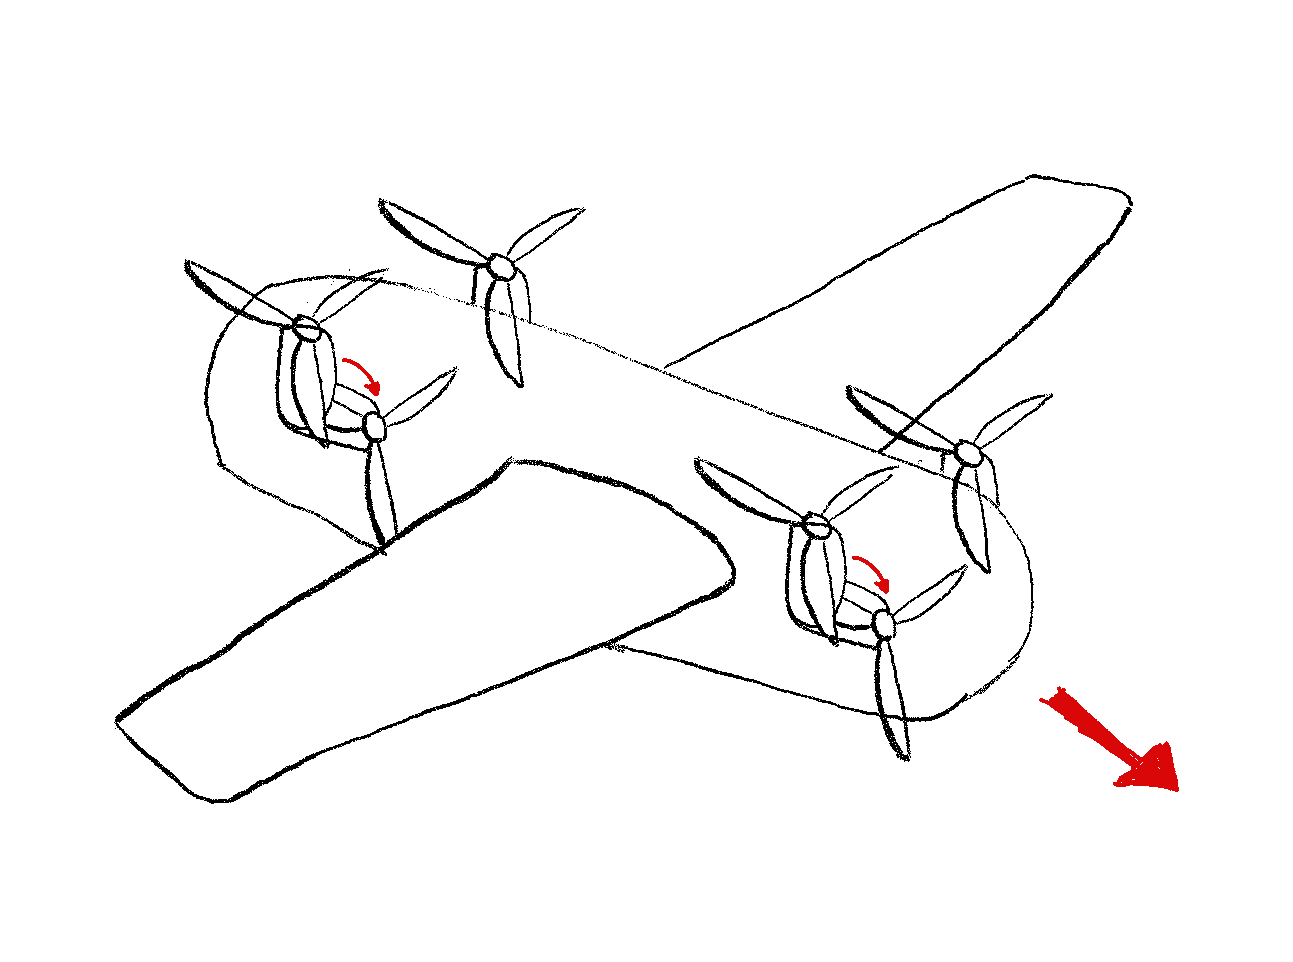
\includegraphics[width=.7\linewidth]{figures/DESIGN_1.png}
  \caption{Concept \ref{C1.5}}
  \label{fig:Concept_C1.5}
\end{subfigure}%
\begin{subfigure}{.5\textwidth}
  \centering
  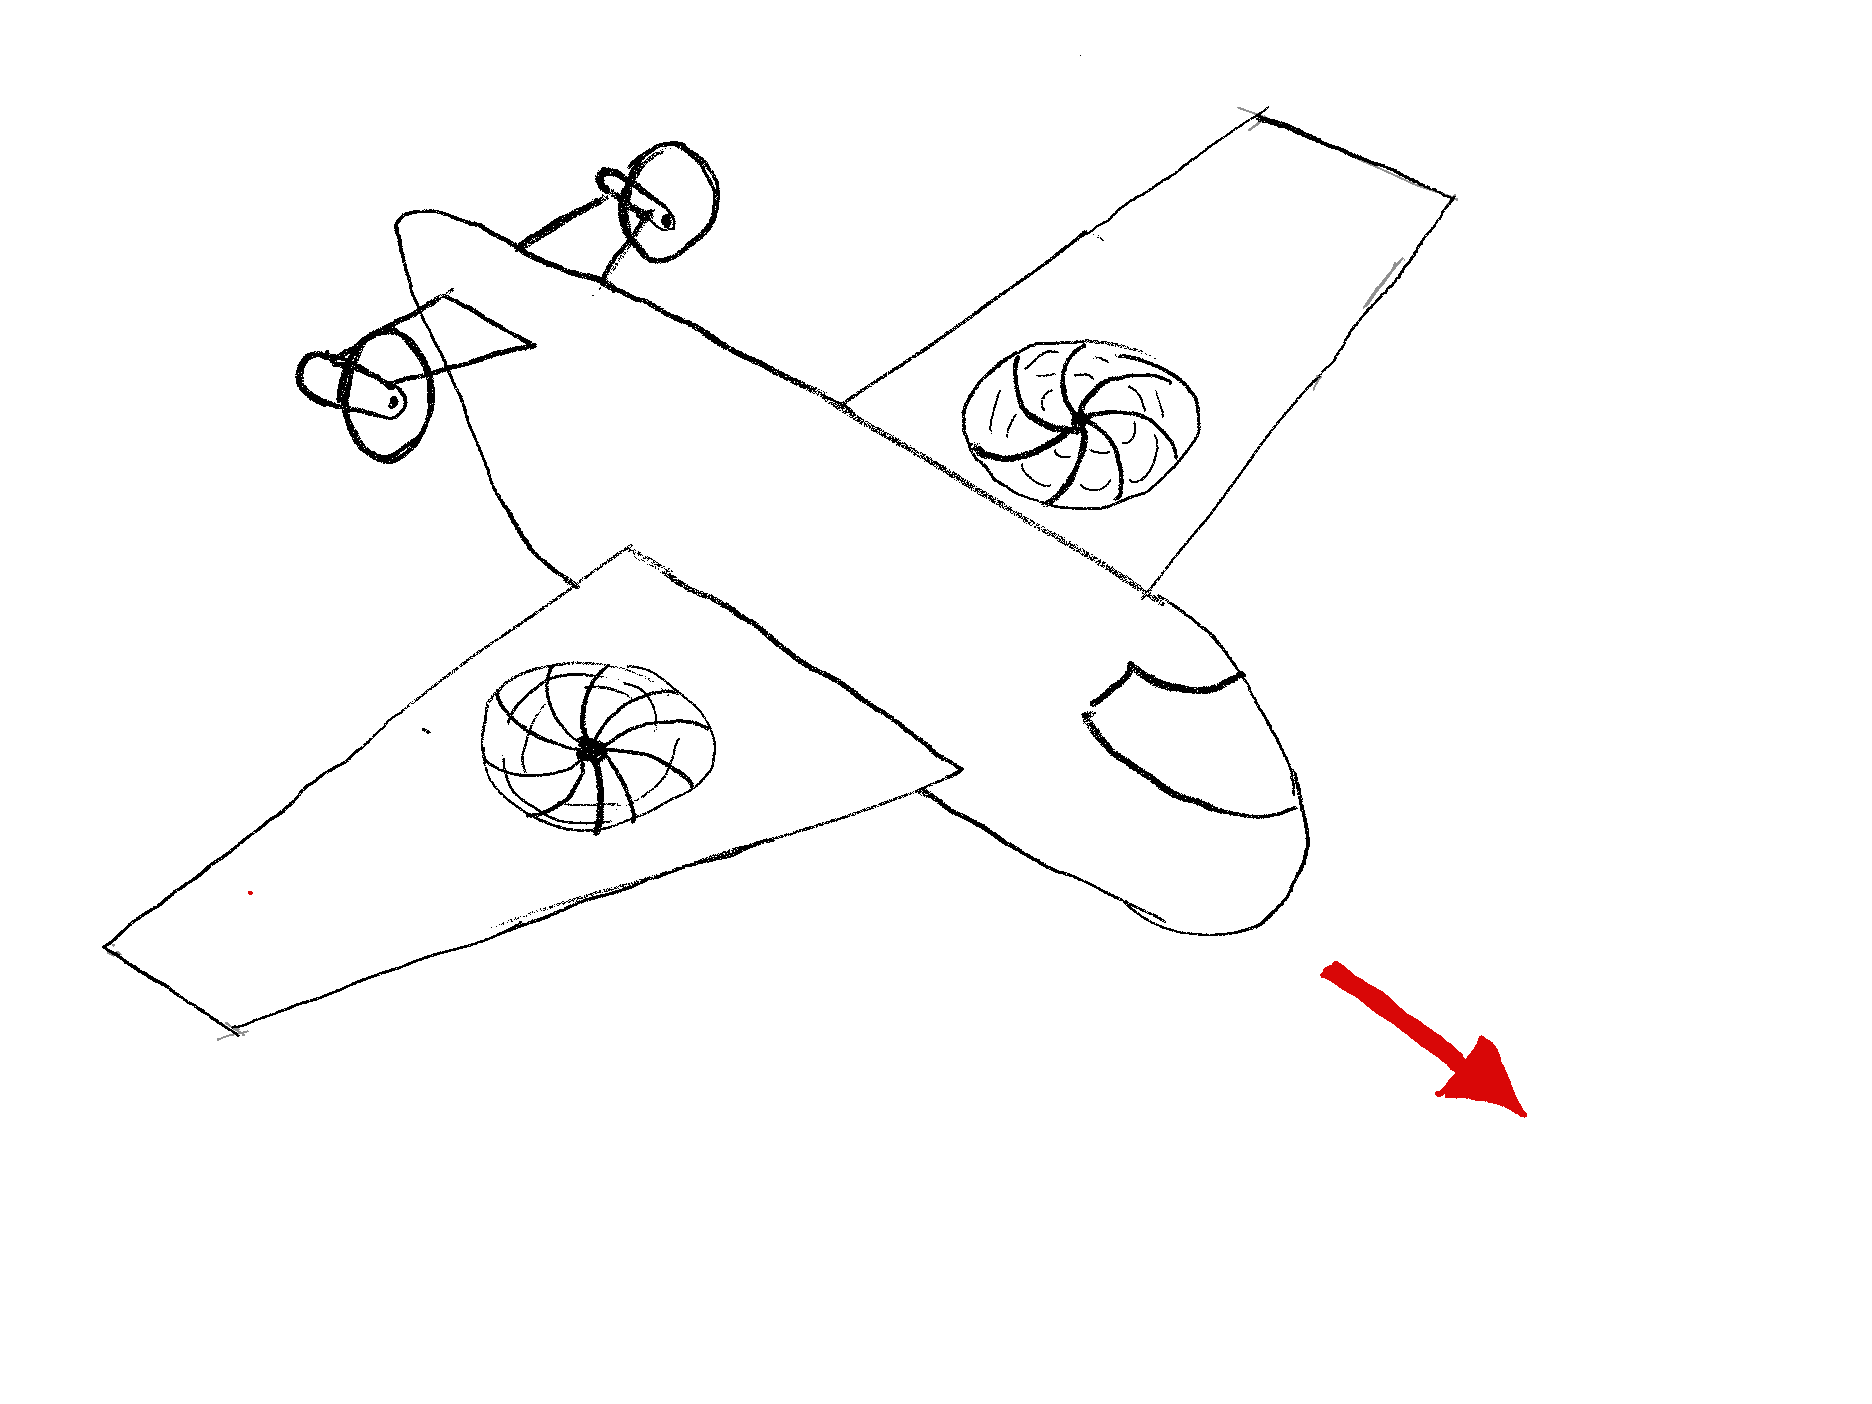
\includegraphics[width=.7\linewidth]{figures/DESIGN_6.png}
  \caption{Concept C1.7}
  \label{fig:Concept_C1.7}
\end{subfigure}
\caption{Concepts of fixed wing structure}
\end{figure}




\section{Transwing}
\label{sec:DesignOptions_Transwing}
Another design option that is relevant in the development of a successful reduced ground footprint VTOL, is the transwing concept.
In this case, the wing is translated and rotated around the body axis of the aircraft, in order to minimise ground footprint while maximising the aerodynamic characteristics of the VTOL vehicle to be designed.
Another concept that can be employed is extending the wings in flight.
 As such, superior range characteristics can be obtained while making sure that the vehicle still respects the requirements, with regard to ground footprint as stated in \Cref{ch:requirements}.

In the case of the transwing concept, several configurations can be conceptualised based on the type of propulsion system and the characteristics of the wing.
Thus, as it can be noticed in the DOT, the transwing concept can be categorised based on two main categories, fixed propulsion or rotating (moving) propulsion.

\subsection{Fixed Propulsion}
The first category, when fixed propulsion is considered, can be further detailed depending on the position of the engines (whether they are situated on the wing or on the fuselage).
In the case of the fuselage-mounted engine, configuration~\ref{C2.10} can be proposed (\enquote{Fuselage mounted propulsion in multiple directions with rotating wings}). This configuration is feasible and as such shall be presented in \Cref{fig:Concept_C2.10}.

When it comes to wing-mounted propulsion, only rotating wings are considered in order to enable the vertical take-off and landing phase of the mission profile.
As such, several configurations can be considered based on the number of wings present in the design and the wing mechanisms employed.
As such, the following configurations are considered: single wing, two wings and telescopic wing.

In the case of the multiple-wing design choice (C2.2) there are some significant drawbacks to the configuration.
Since one wing is placed in front of the other, which implies that the second wing experiences severe down-wash (since both wings will have similar dimensions due to ground footprint requirements).
As such, the benefit of additional lift will be counteracted by the additional drag and reduced velocity on the second wing.
This coupled with the considerable added structural weight leads to an elimination of the concept, due to low performance and significant weaknesses compared to other concepts.

Another possible solution would be the use of telescopic wings to significantly increase the wingspan of the aircraft in the cruise phase, while respecting ground footprint requirements (Concept C2.3).
However, in this particular configuration, it would be very difficult to include ribs within the design, due to the presence of the second part of the wing within the base segment.
As such, to ensure structural integrity and ensure that the stresses and strains within the wing stay within desired values, significantly increased wing skin thickness shall be compared to other configurations.
As such, the design will experience a considerable weight increase compared to other proposed configurations.
Based on this, the configuration was eliminated due to reduced performance compared to other concepts.

Lastly, a single-wing configuration was considered (Concept C2.1).
This concept has been determined to be feasible, since the engines rotate at the same time as the wing.
As such during the VTOL phase, the wing is pointing upward along with the engines.
After the transition phase is reached, the wing rotates around the body axis to enable the engines to point forward.
Afterwards, the aircraft continues flying in cruise configuration, which is identical to a conventional aircraft configuration.
The disadvantage of this concept is the difficulty in rotating the wing around all three axes and the difficulty in ensuring controllability and stability during the transition phase.
However, a possible solution would be to use rotating engines to minimise the impact of the wing transition on the stability of the aircraft, and as such Concept~\ref{C2.5} has been merged into this concept (the only difference being moving propulsion).
This second considered concept shall be showcased in \Cref{fig:Concept_C2.1} for clarity.

\begin{figure}[ht]
\centering
\begin{subfigure}{.5\textwidth}
  \centering
  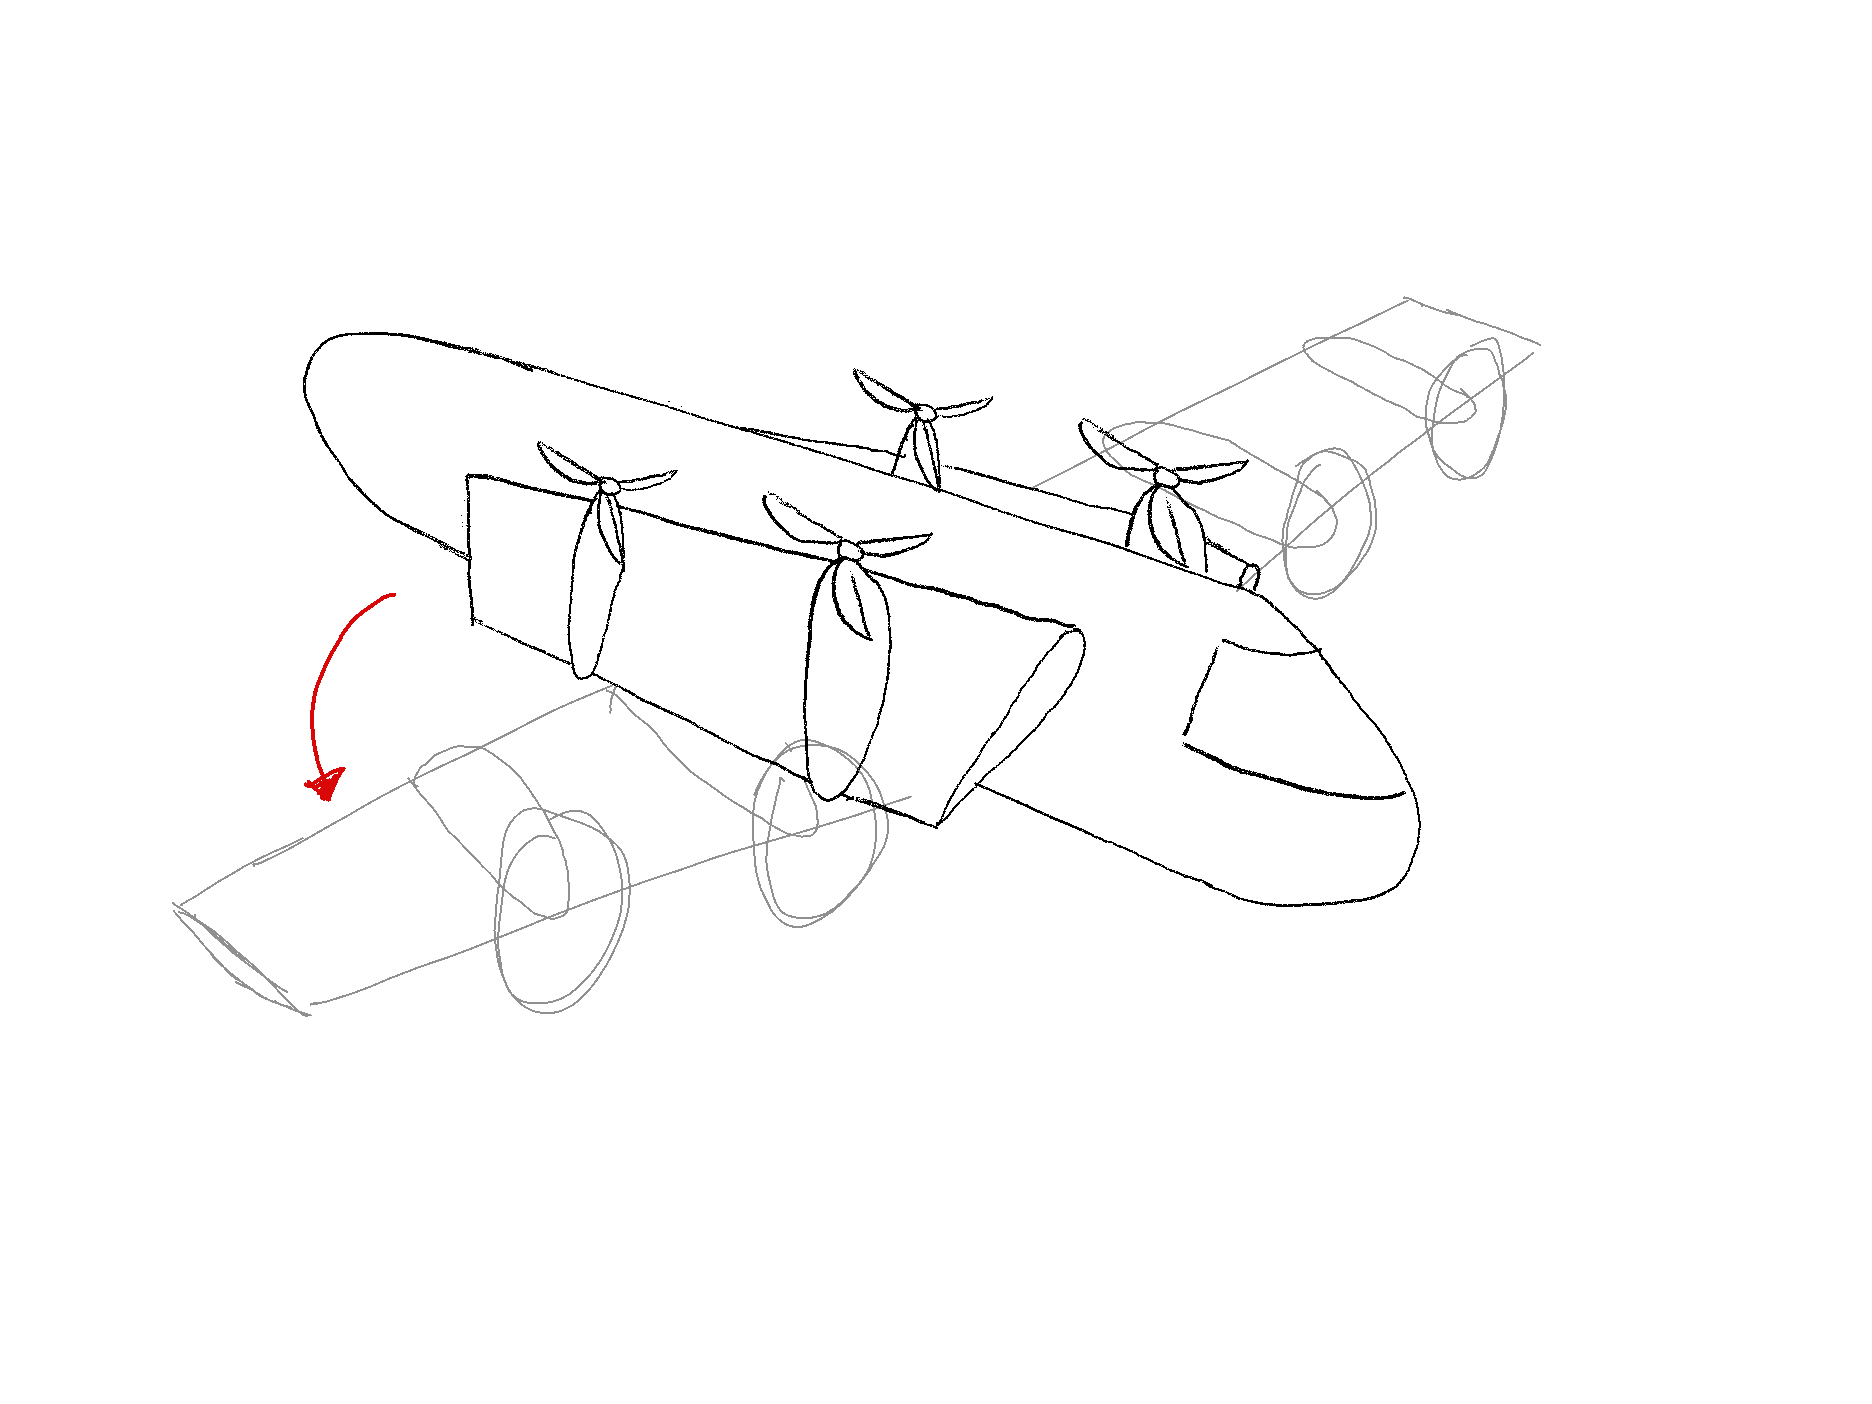
\includegraphics[width=.7\linewidth]{figures/DESIGN_2.png}
  \caption{Concept \ref{C2.1}}
  \label{fig:Concept_\ref{C2.1}}
\end{subfigure}%
\begin{subfigure}{.5\textwidth}
  \centering
  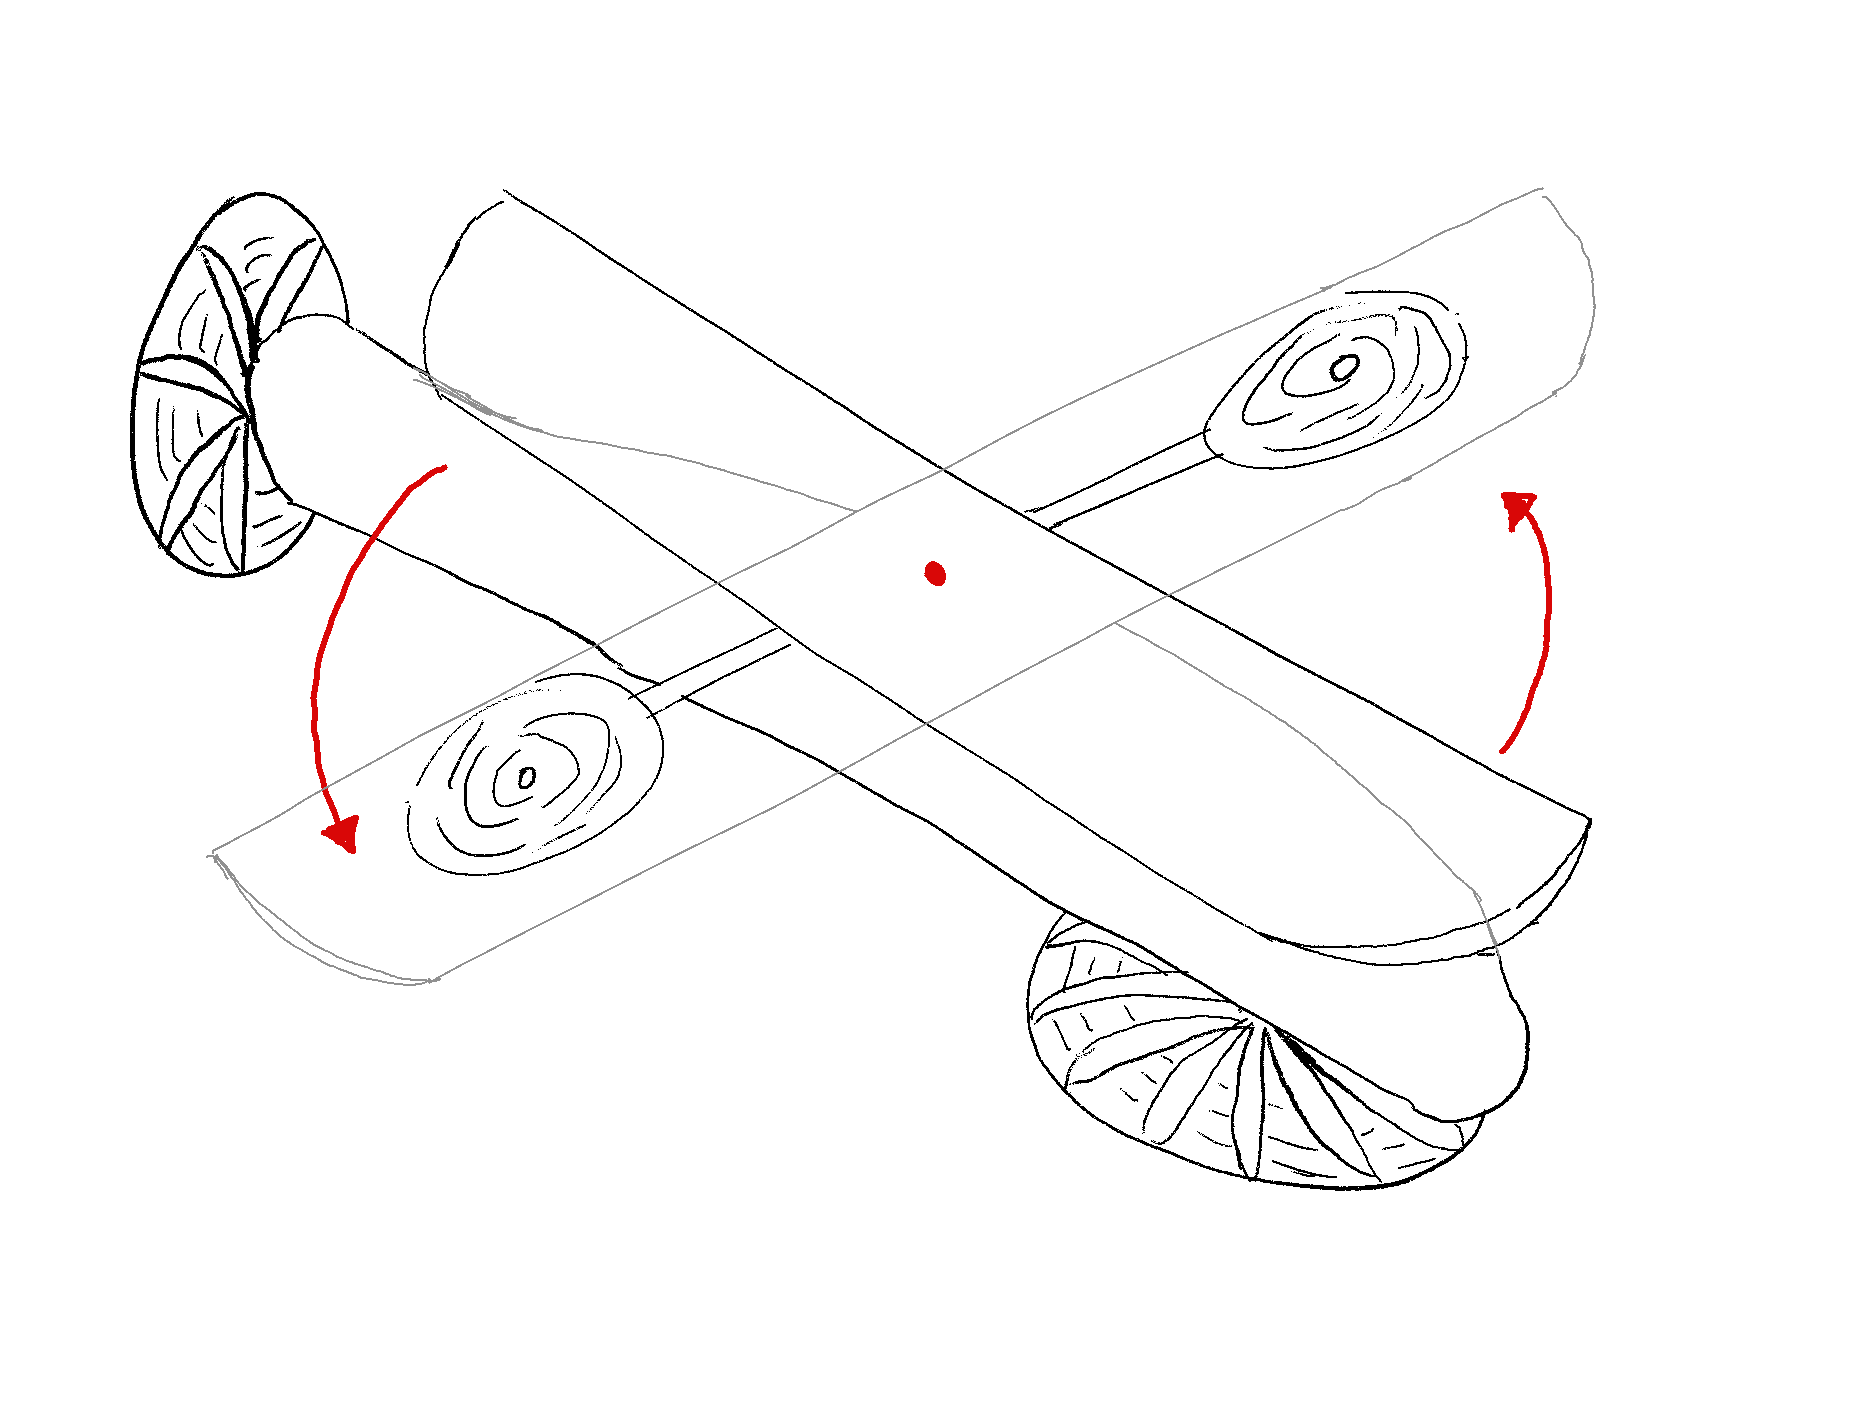
\includegraphics[width=.7\linewidth]{figures/DESIGN_3.png}
  \caption{Concept C2.10}
  \label{fig:Concept_C2.10}
\end{subfigure}
\caption{Concepts of trans wing structure}
\label{fig:drawings_part_2}
\end{figure}
% \begin{figure}[ht]
% \centering
% \begin{subfigure}{.5\textwidth}
%   \centering
%   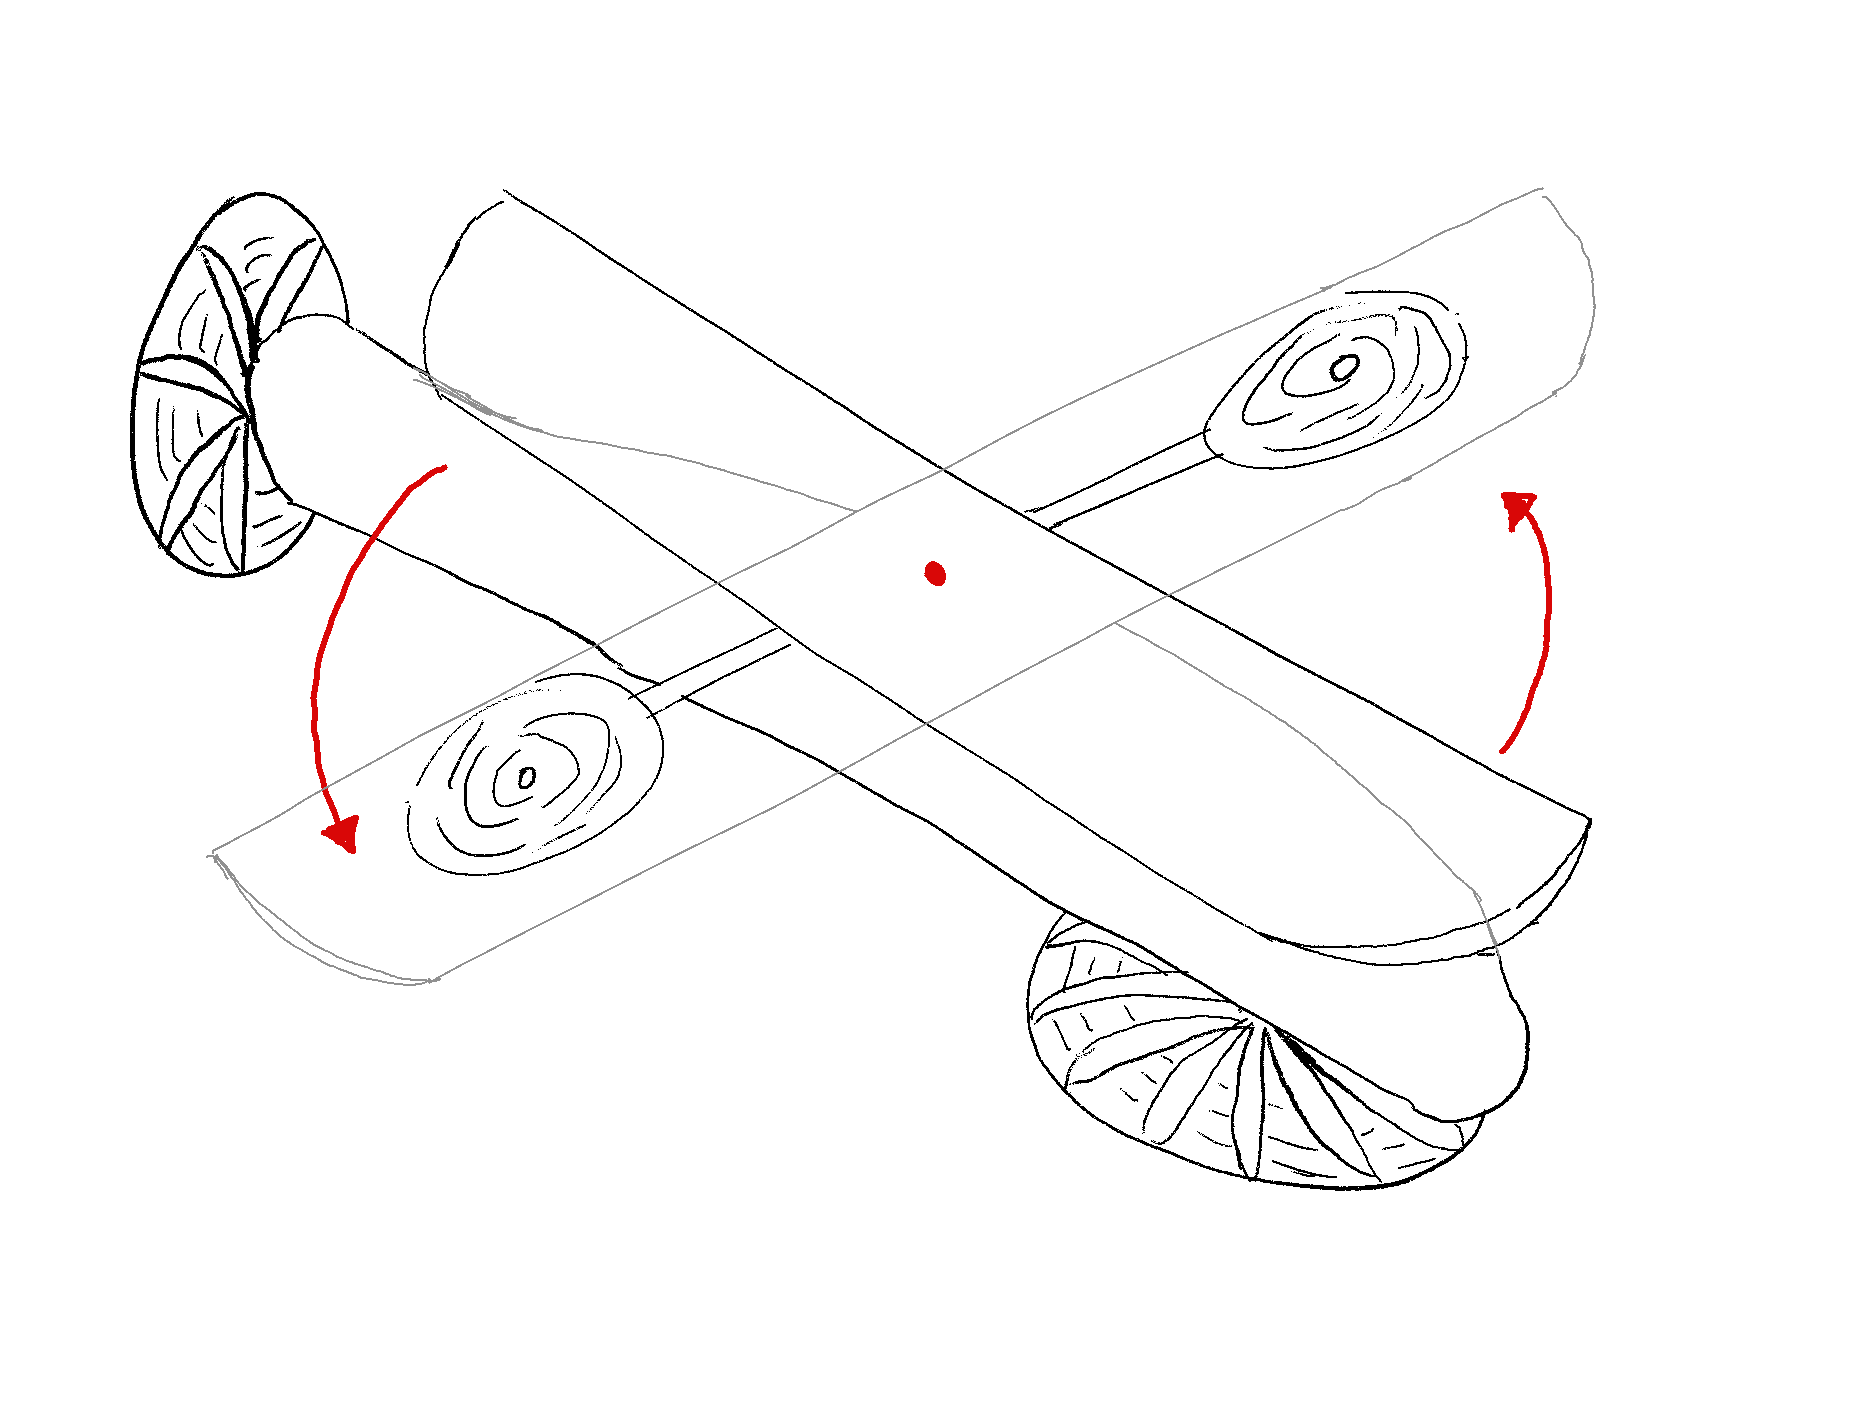
\includegraphics[width=.7\linewidth]{figures/DESIGN_3.png}
%   \caption{test}
%   \label{fig:sub1}
% \end{subfigure}%
% \begin{subfigure}{.5\textwidth}
%   \centering
%   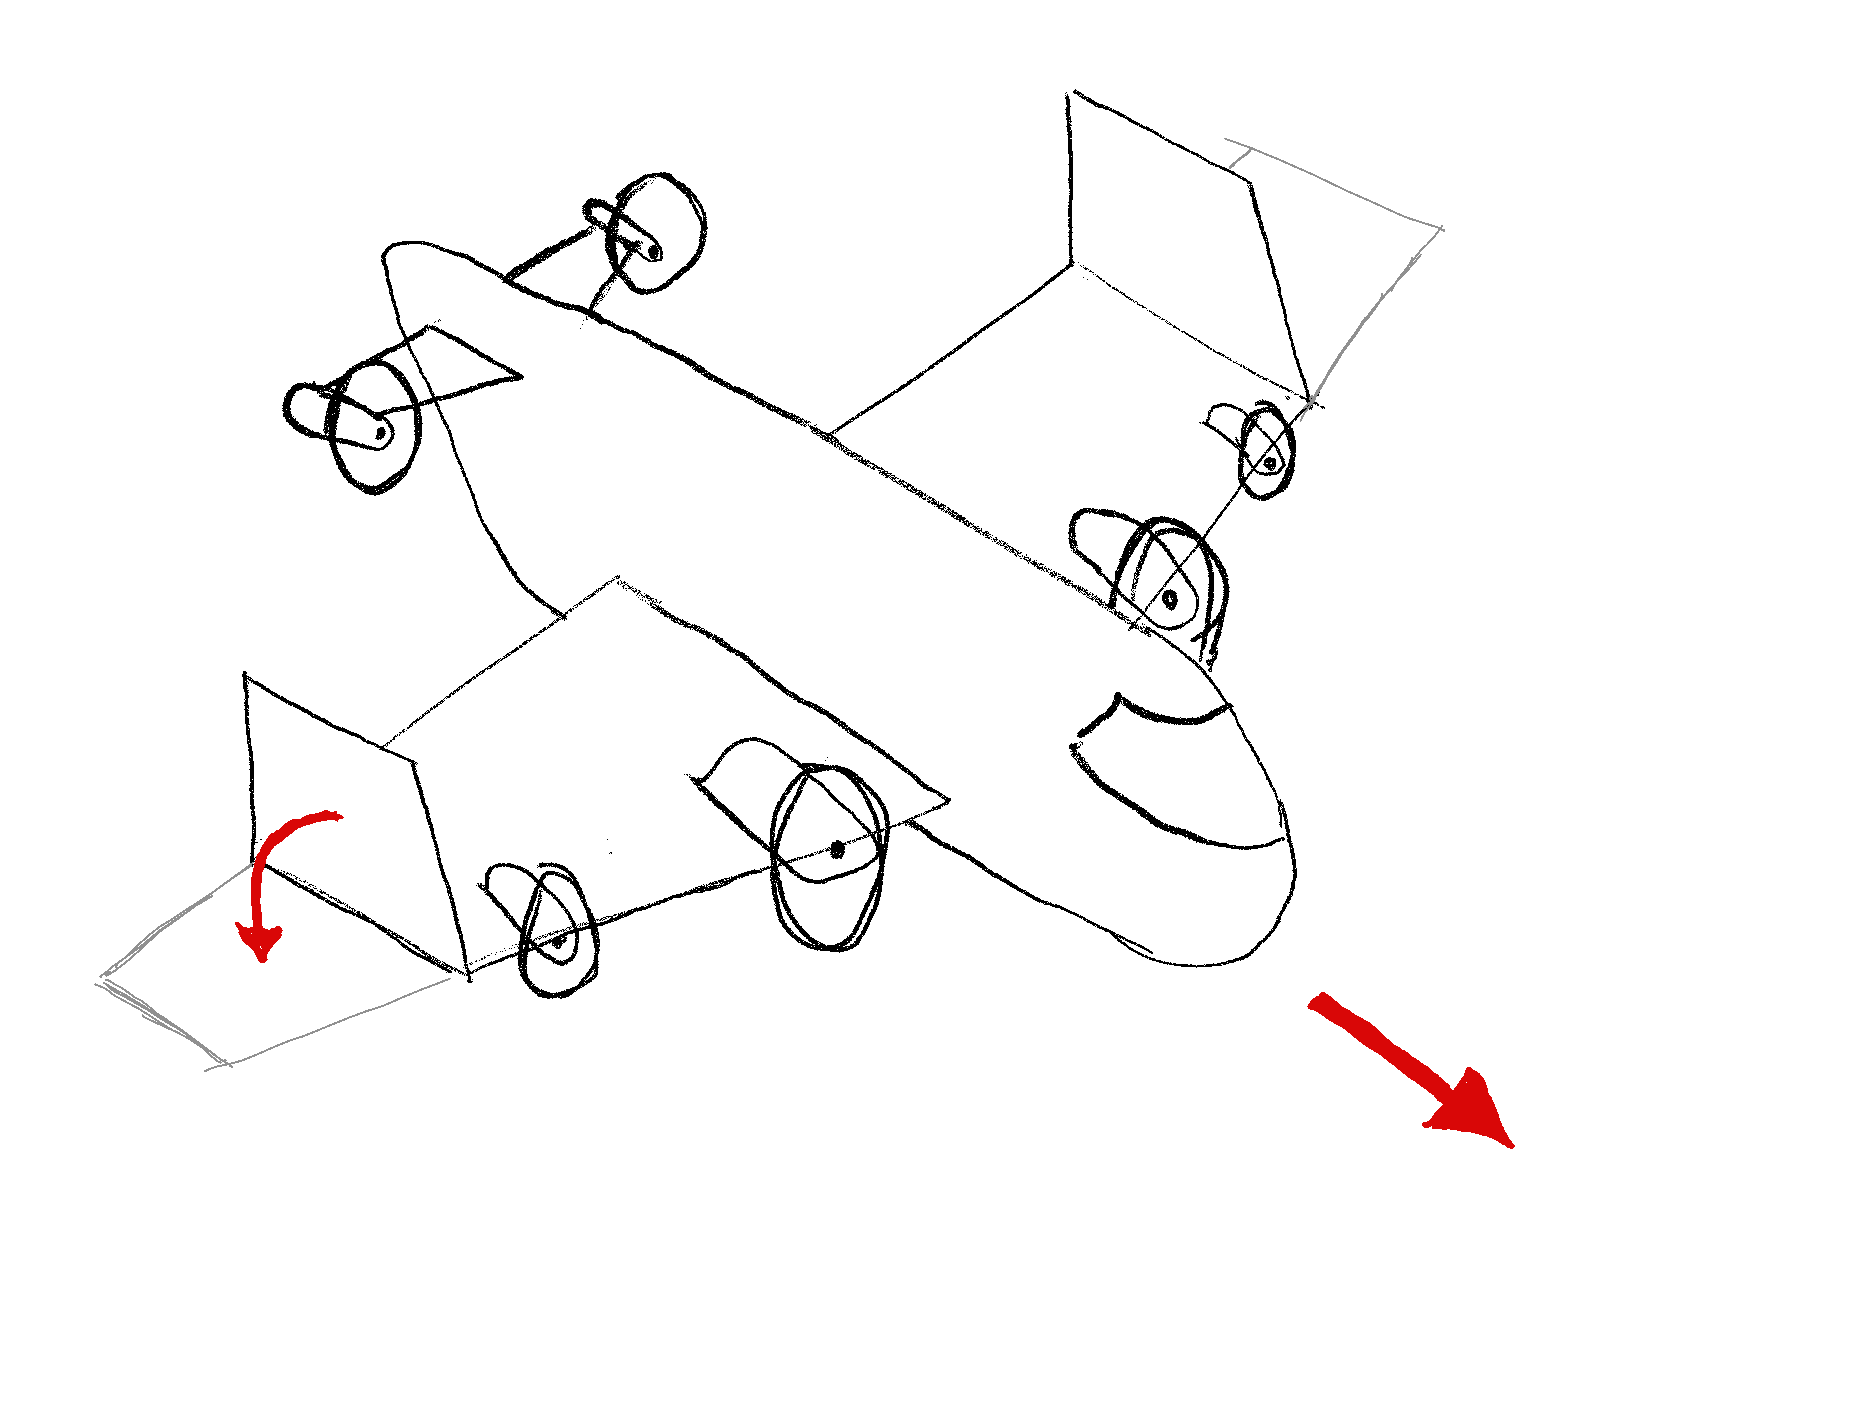
\includegraphics[width=.7\linewidth]{figures/DESIGN_5.png}
%   \caption{test}
%   \label{fig:sub2}
% \end{subfigure}
% \end{figure}
% \todo{ADD DRAWING TIM}


\subsection{Moving Propulsion}
When it comes to rotating/moving engines, several aspects have to be considered when developing design configurations.
As such, the position of the engines has been analysed, as well as the mechanism of the wing transition.
Thus, this design option branch shall also be split into wing-mounted engines and fuselage-mounted engines, based on which several wing configurations shall be proposed.

In the case of the wing-mounted propulsion, several wing configurations have been considered.
In the case of the rotating wing configuration (Configuration C2.5), this configuration has been assumed to be very similar to Configuration C2.1 and as such has been merged into that particular feasible configuration.

Another solution would be using telescopic wings (C2.4).
However, compared to rotating wings, the wing would require additional structural reinforcements in the form of increasing wing skin thickness due to a lack of space for wing ribs.
This configuration was assumed to have severe weaknesses compared to other feasible configurations, and as such has been excluded from the final analysis.

One more possible configuration would be the use of folding wings to enable a reduced ground footprint (Configuration C2.6).
This concept has also been considered feasible and shall be presented in \Cref{fig:Des_5}.

\begin{figure}[H]
    \centering
    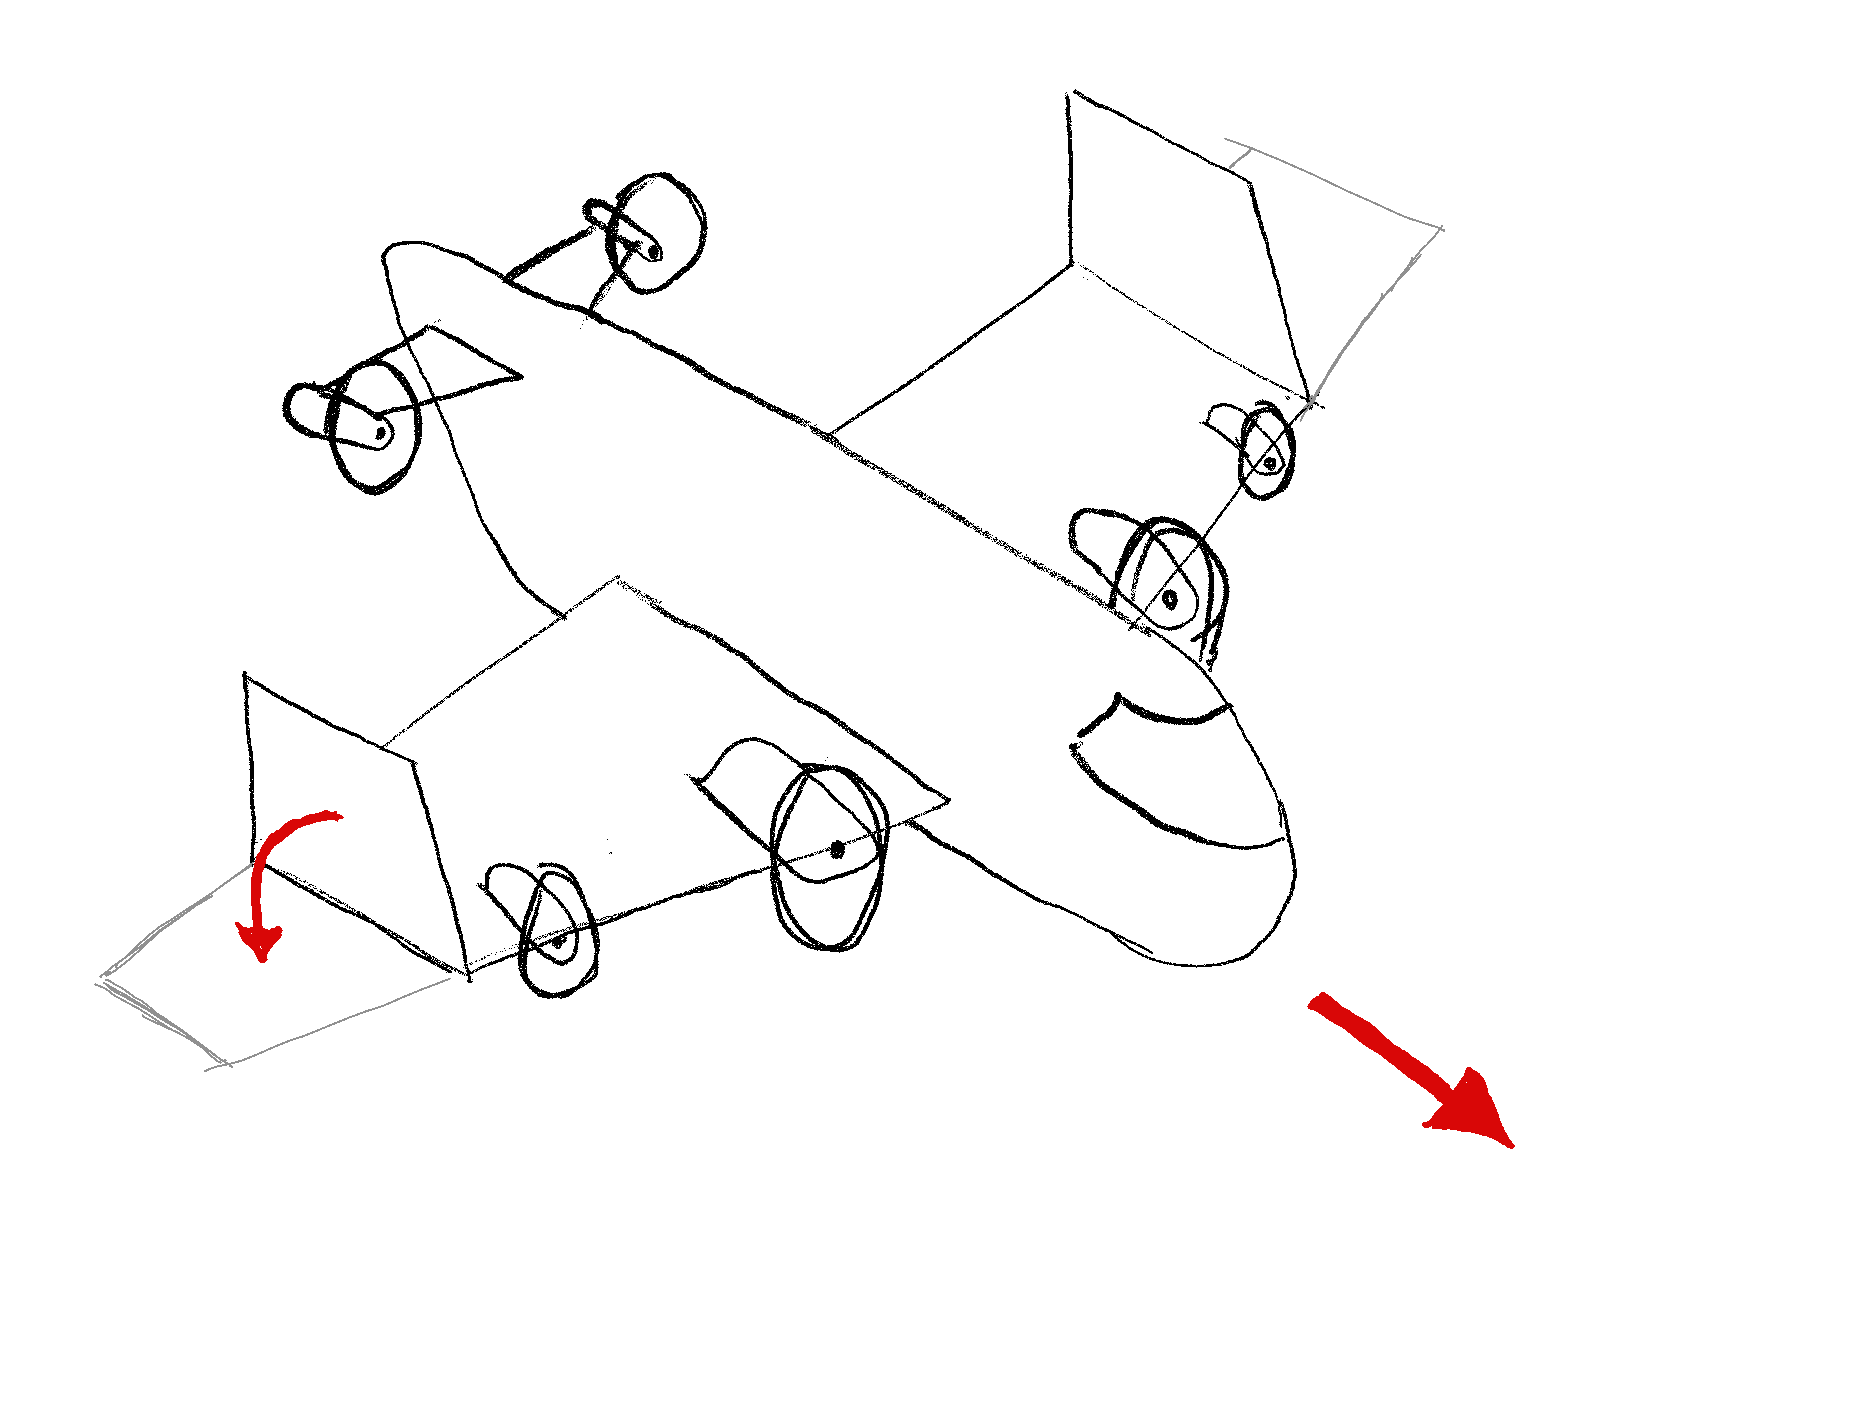
\includegraphics[width=.5\linewidth]{figures/DESIGN_5.png}
    \caption{Configuration C2.6}
    \label{fig:Des_5}
\end{figure}

The last possible configuration to be considered is a sliding wing configuration (C2.7).
However, this would imply the presence of a fixed element that would lead to a decrease in aerodynamic efficiency, thus increase in drag, as well as an increase in complexity due to requiring the design of a roller system along the fixed element, which would be required in order to transition the aircraft from biplane to single wing configuration.
As such, this configuration has been considered unfeasible to design within the scope and time frame of this project, however, this may prove to be a useful idea in subsequent design projects.

For the case of fuselage-mounted propulsion, a telescopic wing as well as a rotating wing configuration have been conceptualised(C2.8;C2.9).
However, both options provide no advantages compared to wing-mounted engine configurations, while having an increase in weight for the telescopic wing and an increase in complexity, due to the required hinge mechanisms for attaching the engines to the fuselage.




\section{Rotorcraft}
\label{sec:DesignOptions_Rotorcraft}
The next main branch of the DOT is the rotorcraft configuration.
A variable disk plane angle is selected for all the options of this branch to ensure the availability of all six degrees of freedom during flight.
The reduction of the ground footprint is not one of the main concerns as hovering and forward flight of rotorcraft do not require a large propeller radius.
Therefore, both fixed and moving arm options can be considered.
Furthermore, moving arms can be subdivided by the type of movement resulting in rotating and telescopic arms.
Optionally, the arm of the rotorcraft can act as a lift-generating device possibly enhancing the range performance of the vehicle.
The combination of the following ideas led to concepts from C3.1 to C3.5.

Subsequently, a brief analysis was performed to assess the feasibility of the rotorcraft configuration.
The market analysis in \Cref{sec:competition-analysis} concluded that the current state-of-the-art rotorcraft market competitors do not meet the range requirement of~\ref{Co-5-STK16-1-1}.
Therefore, the scope of the analysis targets the maximum achievable range of this configuration.

To perform a simplified feasibility analysis, the following assumptions are considered:

\begin{itemize}
    \item The power required for forward flight is identical to the power required for hovering flight.
    \item The power required for hovering flight is given by $P_\text{hov} = \frac{W}{M}\sqrt{\frac{W}{2\rho\pi (n R)^2}}$, where $M$ is the figure of merit, $n$ is the number of rotors, and $r$ is the radius of one rotor~\cite{helicopter_dynamics}.
    \item The number of rotors is 4.
    \item The figure of merit is assumed to be $0.75$~\cite{Figure_of_merit}.
    \item The maximum possible rotor radius implied by~\ref{Co-4-STK13-1-4} is $0.8$ m.
    \item The estimated MTOW of a four-passenger vehicle is $1500$ kg (Prosperity I~\cite{prosperity}).
    \item The rotorcraft is battery-powered and the state-of-the-art battery energy density is $230$ Wh/kg~\cite{Batery_Density}.
    \item According to~\ref{Te-2-STK07-3-2} the cruise speed is $200$ km/h.
    \item According to~\ref{Co-3-STK03-1} the vehicle is capable of flight, thus hovering, with 75\% engine capacity.
    \item The minimum range to be covered is $100$ km (\ref{Co-5-STK16-1-1}).
    \item The electric energy is transformed into mechanical energy with $100$\% efficiency.
\end{itemize}

After summarising the assumptions, the calculation was done by first calculating the required flight time to cover the required range.
Utilising this result and the hovering power the product gives the required energy of $643.4$ MJ. This implies a $777$ kg battery mass using state-of-the-art technology, which is $52$\% of the MTOW. Even though the power required for forward flight is less demanding compared to hovering, this study neglected the required range reserves, vertical take-off and landing phases and the efficiency of the engines~\cite{helicopter_dynamics}.
As a result, the real battery mass is expected to be higher than the preliminary estimate.
Additionally, the lift-generating arms can slightly improve the performance of the configuration.
Yet, it is not expected to improve the range to a feasible extent.
Therefore, the option of pure rotorcraft is discarded and the corresponding branch is pruned from the DOT due to the insufficient technological advancement of battery technologies.

\section{Canard}
The last proposed configuration would be an unconventional canard configuration for the design of the eVTOL, in order to minimise the ground footprint of the design (since no horizontal stabilisers shall be required).
However, canard designs are inherently unstable, and while they do have advantages when it comes to trim drag, the canard proposed configurations would be more useful in the case of designing military UAVs due to high manoeuvrability requirements~\cite{marques2013flight}.
As such, due to the high complexity of the design as well as stability and controllability design issues, this branch has been excluded in its entirety on the basis of too many weaknesses compared to the other alternatives.

\afterpage{
\clearpage
    \KOMAoptions{paper=A3,paper=landscape,pagesize}
    \recalctypearea

    \begin{figure}[p]
    \centering
    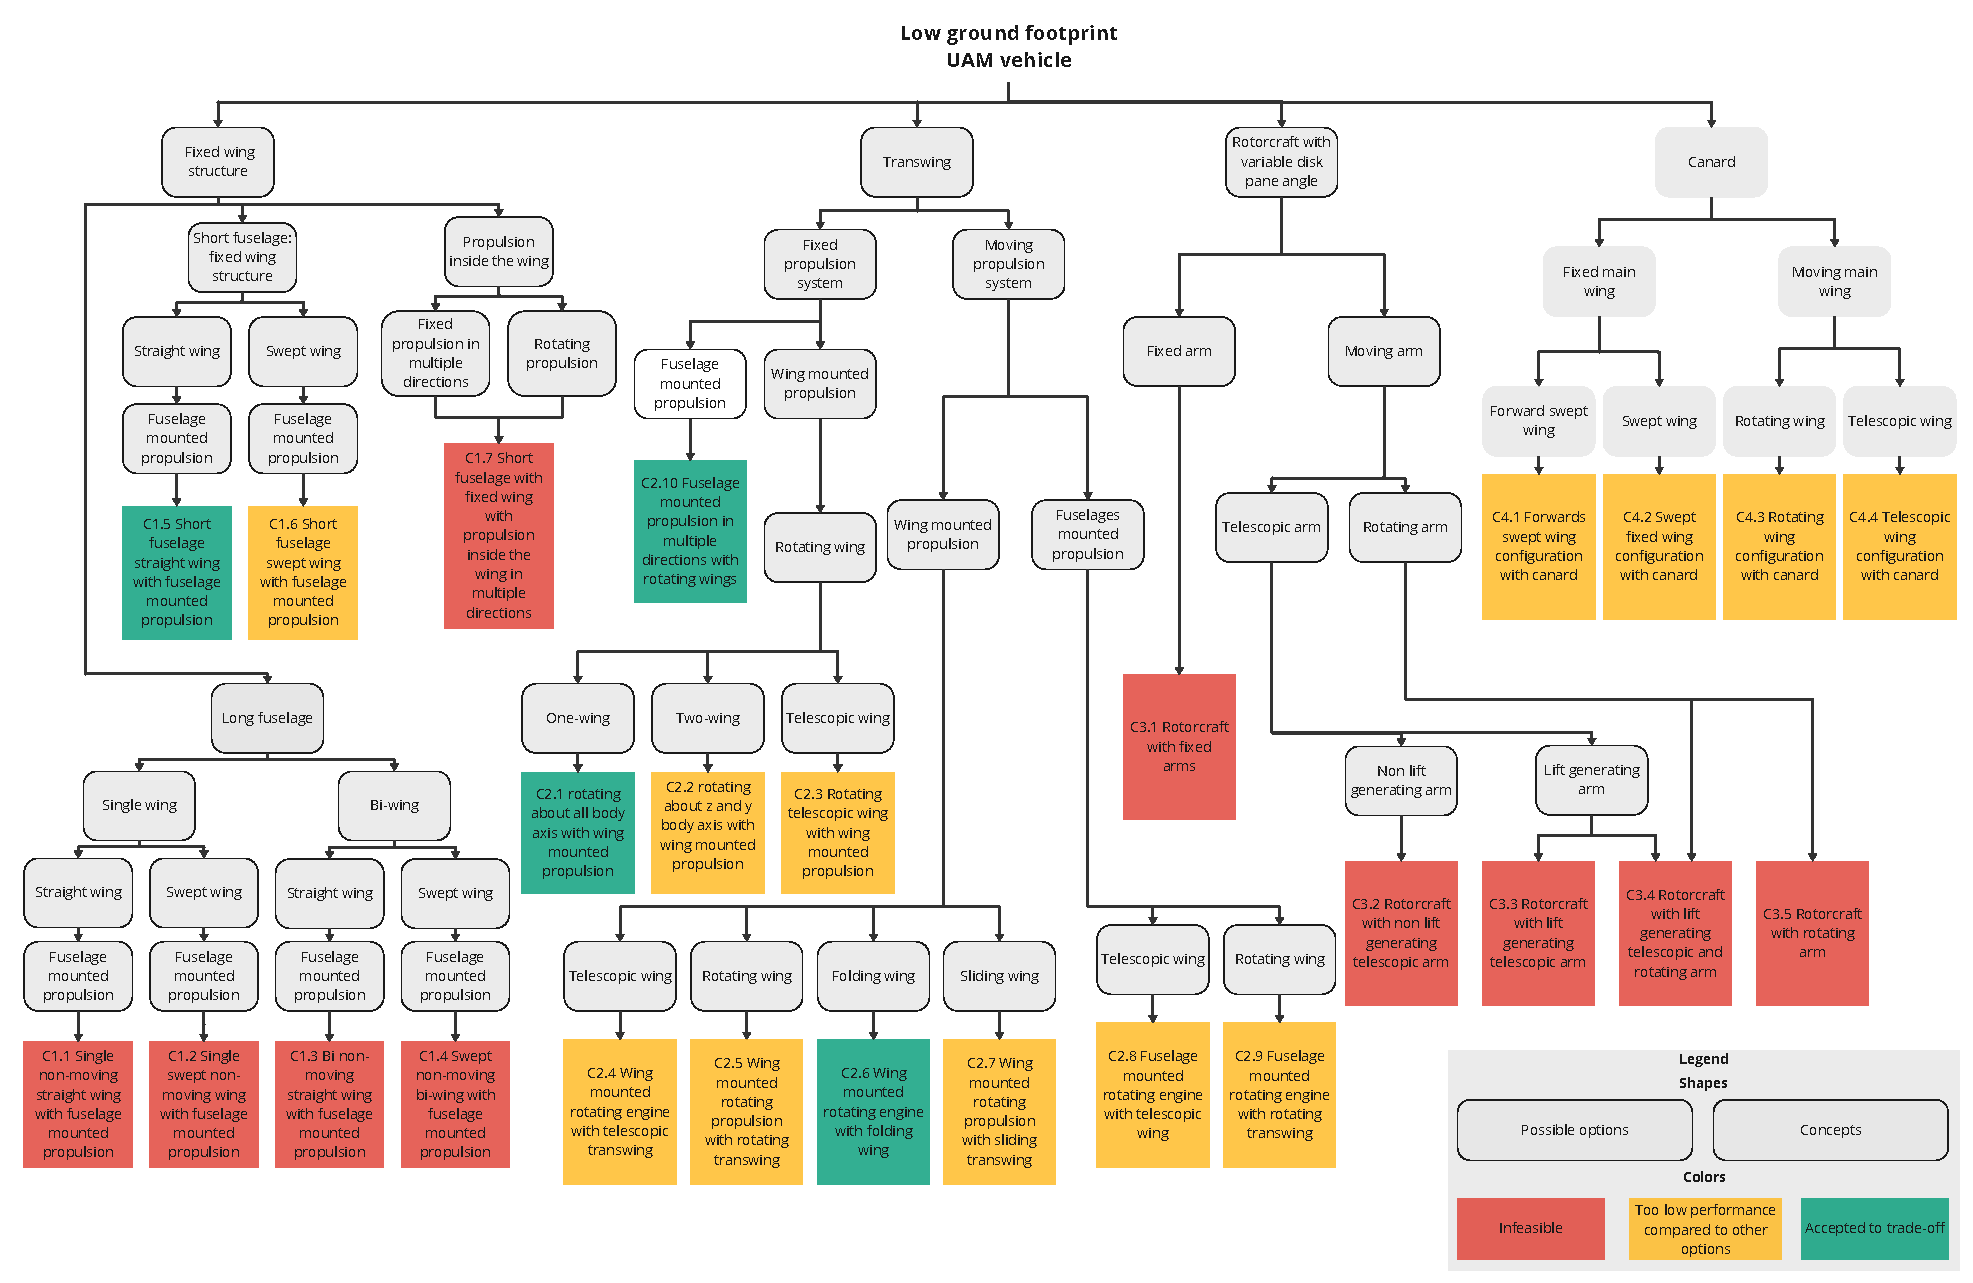
\includegraphics[width=1.1\linewidth]{figures/AE3200 DOT.pdf}
        \caption{Design option three}
        \label{fig:DOT}
    \end{figure}
    
    \clearpage
    \KOMAoptions{paper=A4,paper=portrait,pagesize}
    \recalctypearea
}

